\section{Problem Setting}
\label{sec:problem}

Each contact $v\in V$ specifies satellite $\sigma_v$, ground station
$\gamma_v$, fixed interval $[s_v,e_v)$ and nonnegative reward $w_v$.
Selection reserves the full interval. Source rewards are duration
$e_v-s_v$; synthetic rewards may differ. Configuration $\theta$ fixes pairwise
compatibility throughout a run (Figure~\ref{fig:problem}).

Graph construction is model-specific. For contacts $u,v$ ordered by start
time, a shared ground station creates a conflict when $s_v<e_u+\tau_g$,
where $\tau_g\geq0$ is the station transition time.
Shared-satellite conflicts depend on nonnegative change and transition
thresholds $\tau_c,\tau_t$ and the interval relation.
Source-derived instances retain their declared satellite predicate,
including its admissible crossing overlaps.\footnote{For a common satellite,
equal starts or containment create conflicts. A crossing overlap
$s_u<s_v<e_u<e_v$ conflicts exactly when $e_u-s_v<\tau_c$;
nonoverlapping intervals conflict when $s_v-e_u<\tau_t$.}
Synthetic probes use a separately declared single-capacity overlap model.
Interventions preserve the declared model.

The graph $G_\theta=(V,E_\theta,w)$ joins pairs rejected by these predicates.
With $w(I)=\sum_{v\in I}w_v$, contact selection is MWIS:
\begin{equation}
 \max_{\substack{I\subseteq V\\
                 I\text{ independent in }G_\theta}}w(I).
 \label{eq:mwis}
\end{equation}
Feasibility requires all evaluated hard constraints to be pairwise encoded.

A boundary $B=(F,X)$ records previously selected contacts $F$ and explicit
exclusions $X$. It is admissible when $F$ is independent,
$F,X\subseteq V$, and $F\cap X=\varnothing$. Let
$N_\theta(F)=\bigcup_{v\in F}N_\theta(v)$, where $N_\theta(v)$ is the
neighbor set of $v$. The available actions are
\begin{equation}
 R_\theta(B)=V\setminus\bigl(F\cup X\cup N_\theta(F)\bigr).
 \label{eq:residual}
\end{equation}
For a feasible next action $d\in R_\theta(B)$, define its conditional
completion value as
\begin{equation}
 V_\theta(d\mid B)=
 \max_{\substack{I\text{ independent in }G_\theta\\
                 F\cup\{d\}\subseteq I,\ I\cap X=\varnothing}}w(I).
 \label{eq:conditional-value}
\end{equation}
This includes fixed reward and globally compatible future contacts.

Aligned configurations $\theta_0,\theta_1$ change one resource parameter,
sharing contacts, intervals, identities, rewards and an admissible boundary.
Competing $a,b$ are available and adjacent on both sides; other changed
conflicts can alter their completion values.

A frozen $P=(\phi,h)$ assigns a finite score to every available contact,
$h(\phi(G_\theta,R,v))$. The kernel commits an argmax with deterministic ties,
deletes its closed neighborhood and repeats until $R=\varnothing$.
This guarantees a complete feasible selection. Adaptation uses current graph
and permitted resource fields, without online LLM or oracle calls.

\begin{figure*}[tp]
 \centering
 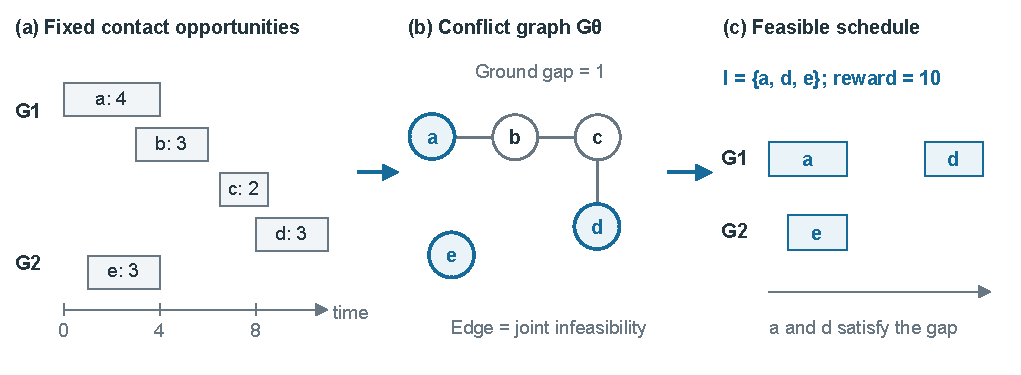
\includegraphics[width=\textwidth]{figures/problem_setting-wide.drawio.pdf}
 \Description{Contact intervals grouped by ground station,
 their weighted conflict graph, and the intervals retained in a complete
 feasible selection.}
 \caption{From contact opportunities to a complete feasible schedule:
 resource predicates create conflict edges; vertex weights encode contact
 rewards; an independent set selects mutually compatible contact intervals.}
 \label{fig:problem}
\end{figure*}
